\documentclass[class=article, crop=false]{standalone}
\usepackage[utf8]{inputenc}
\usepackage{graphicx}
\renewcommand{\baselinestretch}{1.5} 
\usepackage{wrapfig}
\usepackage{subcaption}
\usepackage{caption}
\usepackage{float}
\usepackage{xcolor}
\usepackage{amsmath}
\usepackage{blindtext}
\usepackage{import}
% \usepackage[backend=biber, style=numeric, citestyle=nature, doi=false, isbn=false, url=false, eprint=false]{biblatex} %Imports biblatex package, Comment out main doc
% \addbibresource{refs.bib} %Import the bibliography file, Comment out main doc

\begin{document} 
\label{section:Quad}

\section{Introduction}

\subsection{Quadrupolar Splitting}

Because of deuterium's ($^2$H) nuclear spin (I=1) being larger than 1/2 it possesses an electric quadrupolar magnetic moment (Q$_{\text{deuteron}}=$ 0.286 fm$^2$) \cite{Stone2015NuclearData}. This quadrupolar moment interacts with the local electric field gradients (EFG) which can be represented as a combination of up to six electric potential tensor elements, these aree then simplified to three principal axis elements (V$_{xx}$, V$_{yy}$ and V$_{zz}$). By definition the sum of these elements is 0, as the EFG is a traceless tensor. V$_{zz}$ is defined as the largest element and is usually specified as the EFG at the quadrupolar nucleus (V$_{zz} = e\cdot q$)\cite{Elliott2021WhatMedia}. The ratio of the difference between V$_{xx}$ and V$_{yy}$ to V$_{zz}$ is referred to as the asymmetry parameter ($\eta$).
\begin{equation}
    \eta = \frac{V_{xx}-V_{yy}}{V_{zz}}
\end{equation}
By considering the time-independent Hamiltonian ($H_Q$) of this interaction it is possible to find a mathematical generalised form.
\begin{equation}
    H_Q = \frac{eQ}{4I(2I-1)}[V_0(3I^2_z-\boldsymbol{I}^2) + V_{\pm1}(I_{\mp}I_z+I_zI_\mp)+V_{\pm2}I^2_\mp]
\end{equation}
V$_0$, V$_{\pm1}$ and V$_{\pm2}$ are the three principal axis elements combined to create new elements, which are complex, that better represent the total EFG. When considering the rotational transformation from the molecule's fixed reference frame to the laboratory fixed reference frame\cite{Seelig1977DeuteriumMembranes}, along with an assumed value of $\eta$=0 (uniaxiality), the total Hamiltonian simplifies for deuterium ($I$ = 1) \cite{Sharf1995DetectionNMR-Spectroscopy}. The form of this equation, now using its simplified principal axis elements is:
\begin{equation}
    H = -g\beta_N\boldsymbol{I}\cdot\boldsymbol{H_0} + \frac{eQ(3\cos^2(\theta)-1)}{8}V_{zz}(3I_z^2-\boldsymbol{I}^2)
\end{equation}
where $g$ is the g-factor, $\beta_N$ is the nuclear magneton, Q is the (scalar) quadrupole moment, $\boldsymbol{H_0}$ is the magnetic field, $e$ is the charge of an electron, $I$ is the nuclear spin (of deuterium) and $\theta$ is the angle between the electric potential and the magnetic field. Now that a simplified total Hamiltonian is found the perturbed energy levels can be calculated, which will have an associated energy difference and therefore a frequency difference.
\begin{equation}
    \nu_Q(\theta) = \frac{3}{2}\left(\frac{e^2qQ}{h}\right)\left(\frac{3\cos^2(\theta)-1}{2}\right)
    \label{eqn.Angle}
\end{equation}
where the RQC in this case is given in the first part of the above equation.
\begin{equation}
    \omega_Q/2\pi = \frac{3}{2}\left(\frac{e^2qQ}{h}\right)
    \label{eqn.RQC}
\end{equation}

The above derivation shows that as a result of the quadrupolar magnetic moment interacting with the EFG a splitting is observed that is caused by perturbed energy levels. The frequency magnitude of this splitting effect is quantifiable and depends only on the orientation of the deuterated sample to the applied magnetic field (equation \ref{eqn.Angle}. In an isotropic structure such as the brain this splitting effect is not visible due to averaging resulting from molecular motion. In an anisotropic media such as the skeletal muscle fibres in the calf, the quadrupolar splitting is at a maximum and equal to the RQC value when the deuterated sample is orientated with the magnetic field ($\theta = 0^\circ$). The splitting effect can also be nulled ($\nu_Q = 0$) if the sample is orientated to the magnetic field at the magic angle $\theta = 54.74^\circ$ ($\cos^2\theta=1/3$).

Using an NMR technique known as double quantum filtering (DQF) signals resulting from single and zero quantum coherences are suppressed, leaving only the effect of double quantum coherences. The resulting signal is always a single quantum coherence, therefore the DQF converts the double quantum coherences into single coherence. Any signal detected using a DQF sequence hence proves the existence of double quantum coherences.

This detected signal is related to a second rank tensor arising from the EFG, which can only be formed in anisotropic media/phases. Therefore it is possible to measure the RSC constant from these NMR spectra which provides information on the anisotropy of the media investigated. This technique is applied by manipulating the pulse sequence with alternating $\pi/2$ and $\pi$ RF pulses. By measuring the anisotropy of tissues and fluids in the body such as intervertebral disc tissue \cite{Ooms2015DoubleTissue}, brain water\cite{Assaf1997InSpectroscopy} and elastin\cite{Sun2010InvestigationNMR} reveals a lot about the presence of diseases such as degenerative disc disease\cite{Ooms2015DoubleTissue}.

\subsection{Aims}

During the loading measurements were obtained that were used to measure the dependency of the quadrupolar splitting on the angle orientation of skeletal muscle to the magnetic field, along with implementing double quantum filtered on skeletal muscle at 3T.

\section{Methods}

\subsection{Quadrupolar Splitting}

After the initial D$_2$O loading period was completed and the participants $^2$H enrichment had reached a steady state level. The left calves of participants A and B were scanned again using a Philips 3T Achieva scanner along with an in-house built $^2$H saddle coil (~16 cm diameter). A $^1$H 3D gradient-echo (GE) anatomical image (TE=2.1 ms, $\alpha$=15$^{\circ}$, T$_{scan}$= 122 s, TR=20 ms, FOV=128x128x192 mm$^3$, TR=20 ms, Voxels=2 mm isotropic) was obtained along with a 3D chemical shift image (CSI, NSA=2, 256 samples, TE=6.2 ms, TR=500 ms, BW=750 Hz, FOV=120x120x60 mm$^3$, Voxels=10 mm isotropic). The CSI was originally obtained to look at the overall spread of $^2$H enrichment in skeletal muscle, however quadrupolar splitting was observed across the calf (most notably in the tibialis anterior muslce.) This was used as motivation to investigate the effect of quadrupolar splitting in skeletal muscle.

Participants A and B were therefore scanned again using the Philips 3T Achieva and an in-house built $^2$H coil consisting of two octagonal loops (~14 cm diameter) separated by ~12 cm designed to scan the forearm. The left forearms of A and B were scanned as this allowed us to easily bend the arm in the coil at different angles with respect to the B0 field of the magnet, which allows us to change $\theta$ in equation \ref{eqn.Angle}. A $^1$H 3D GE image (Scan details) was acquired along with a $^2$H 3D CSI (Scan Details) for a range of different arm angles. During scanning, for each angle, participants were lay in a prone position with their left arm above their head. A 'straight' arm represented  0$^{\circ}$ angle respect to the B0 field, participant A was then scanned with angles of 0, 10, 20, 30 and 40$^{\circ}$ in one visit and 50, 60, 70, 80 and 90$^{\circ}$ in a second visit. Participant B was scanned with angles 0, 85, 30, 15, 45, 60, 75 and -10$^{\circ}$ in a single visit. 

The 3D CSI spectra for the forearm was analysed using MATLAB and started with zero-order phase correction and masked based on the maximum value from the spectra of a specific voxel being larger than 20\% of the maximum value of all spectra. Each voxel within the mask was then fit to two complex Lorentzian curves with equal amplitudes, phases and linewidths where the frequency splitting between the two peaks is determined from fitting. The spectra is also fit to three complex Lorentzian curves where the two 'outer' peaks have equal equal amplitudes, phases and linewidths similar to before except now there is a third central peak with different amplitude, phase and linewidth to the other peaks the frequency splitting is now the frequency difference between the 'outer' two peaks only. The fitting is performed by minimising the sum of the squared difference between the proposed fit and the phase-corrected signal, this was done using in-built MATLAB function fmincon. The best fit is determined by comparing the final minimised value returned from fitting, whichever combination of Lorentzian curves gave the lowest value is kept and outputted for that voxel. The frequency splittings are then averaged over the masked region to give a single frequency splitting for that angle. This process was repeated for each angle. All the splitting's were then fit to equation \ref{eqn.Angle}, where the total RQC is determined. This was repeated for participants A and B.

\section{Results}

\subsection{Quadrupolar Splitting}

\begin{figure}
    \centering
    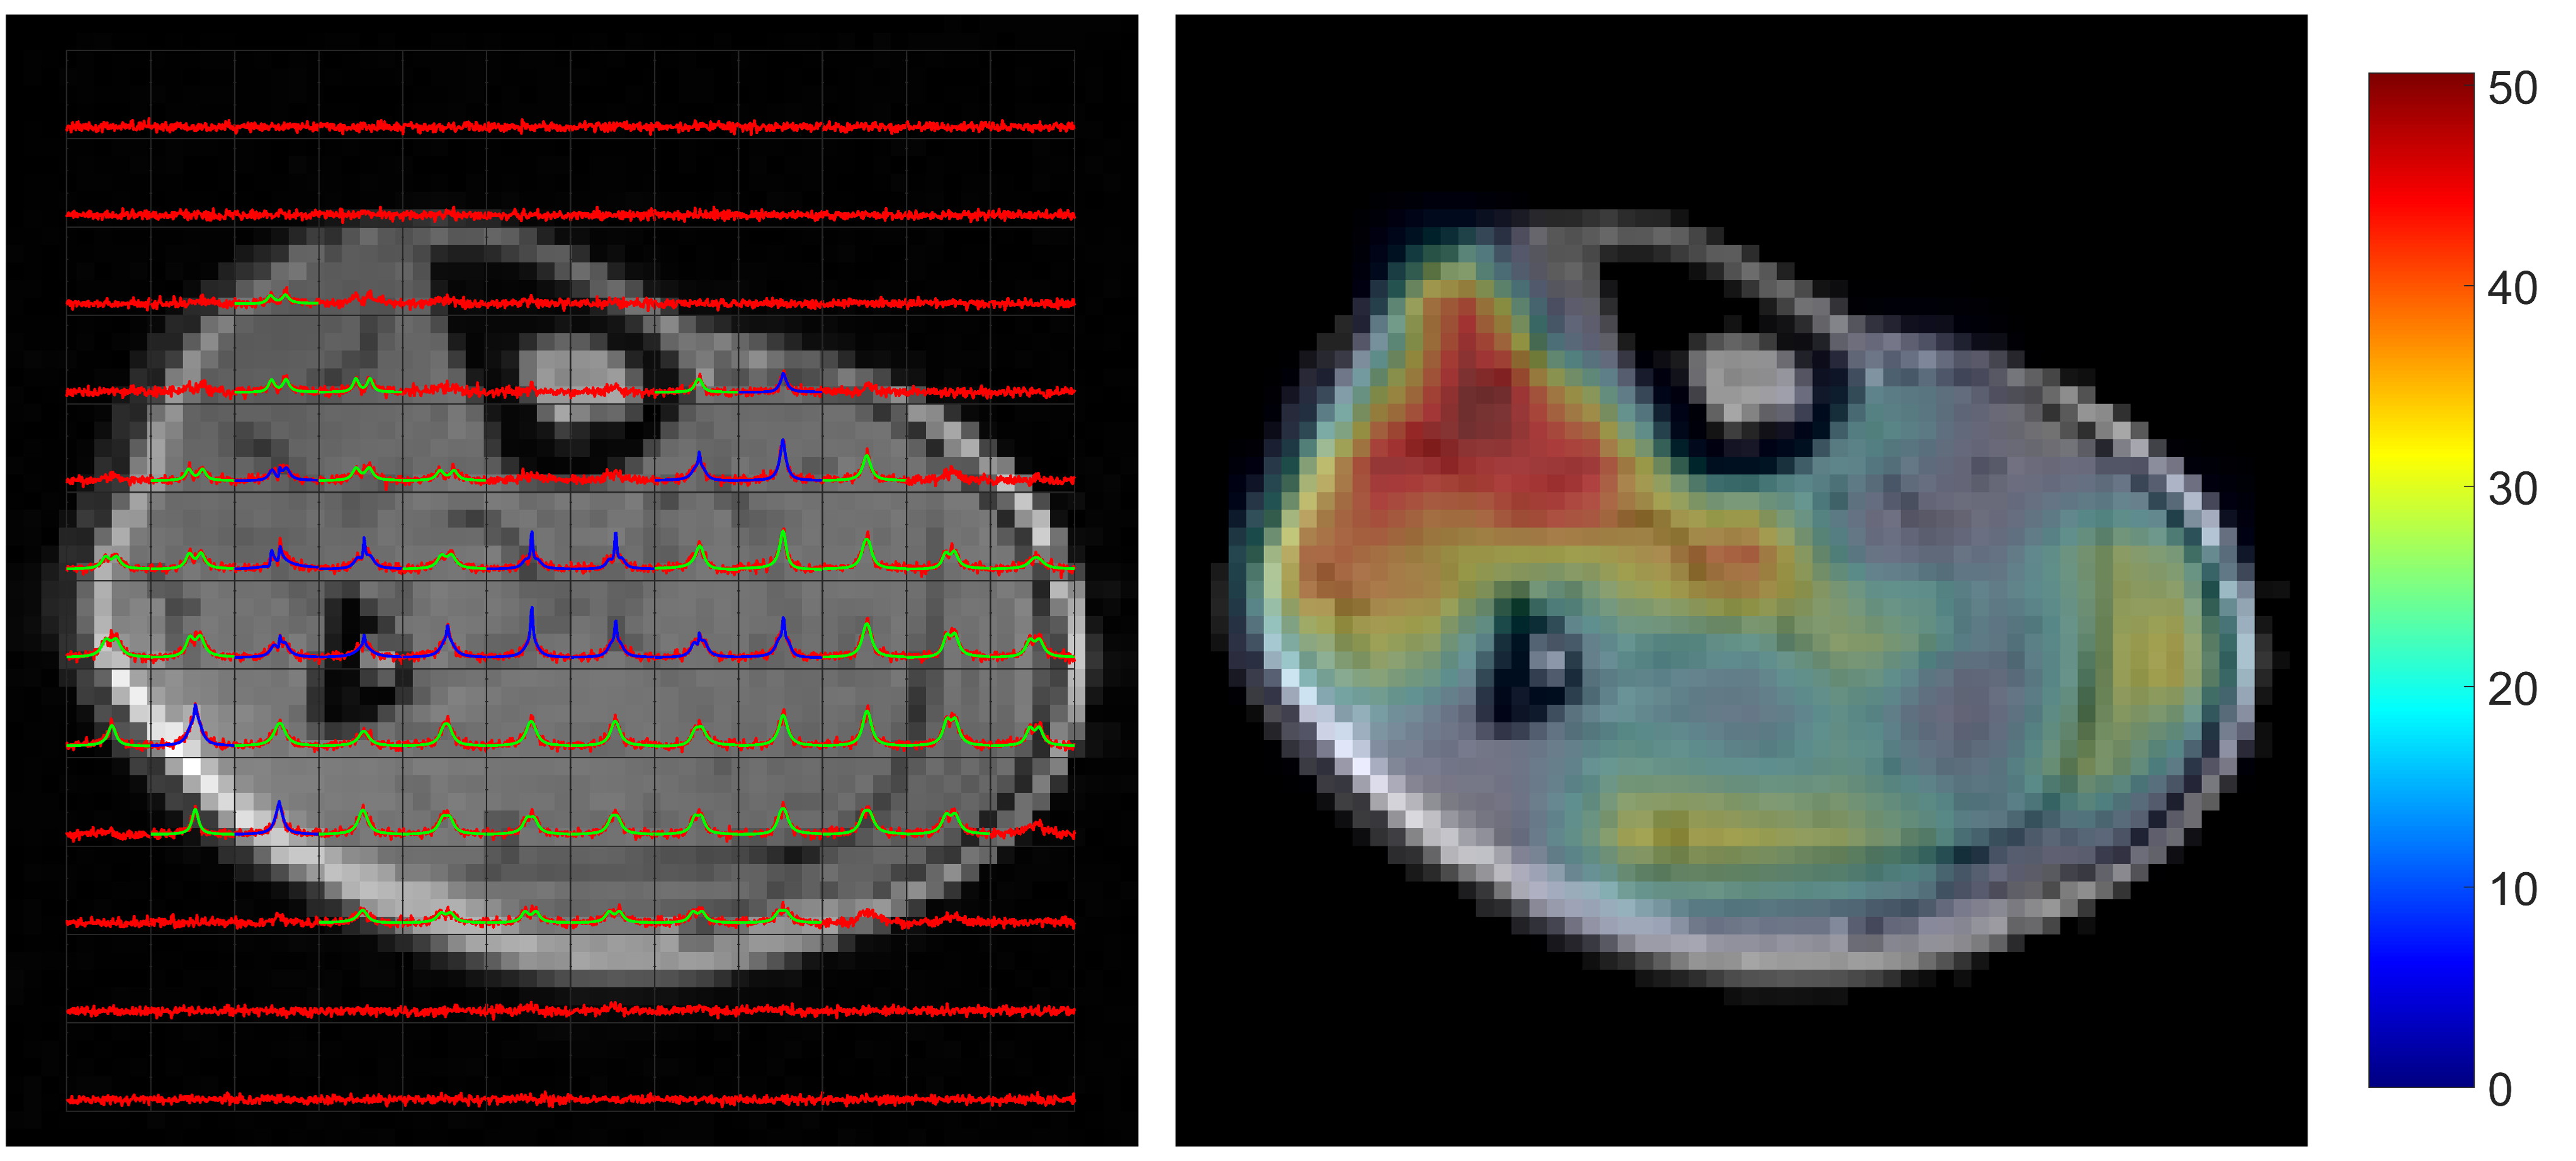
\includegraphics[width=1\textwidth]{Figures/D2O/Calf_A.png}
    \caption{Left: CSI spectra (red) overlayed onto a $^1$H GE image from participant A's left calf of a single slice, with fits of two Lorentzian peaks (green) and three Lorentzian peaks (blue). Right: Interpolated map of quadrupolar frequency splitting's overlayed onto the same $^1$H GE image from participant A's left calf. }
    \label{fig:D2O:Calf_A}
\end{figure}

\begin{figure}
    \centering
    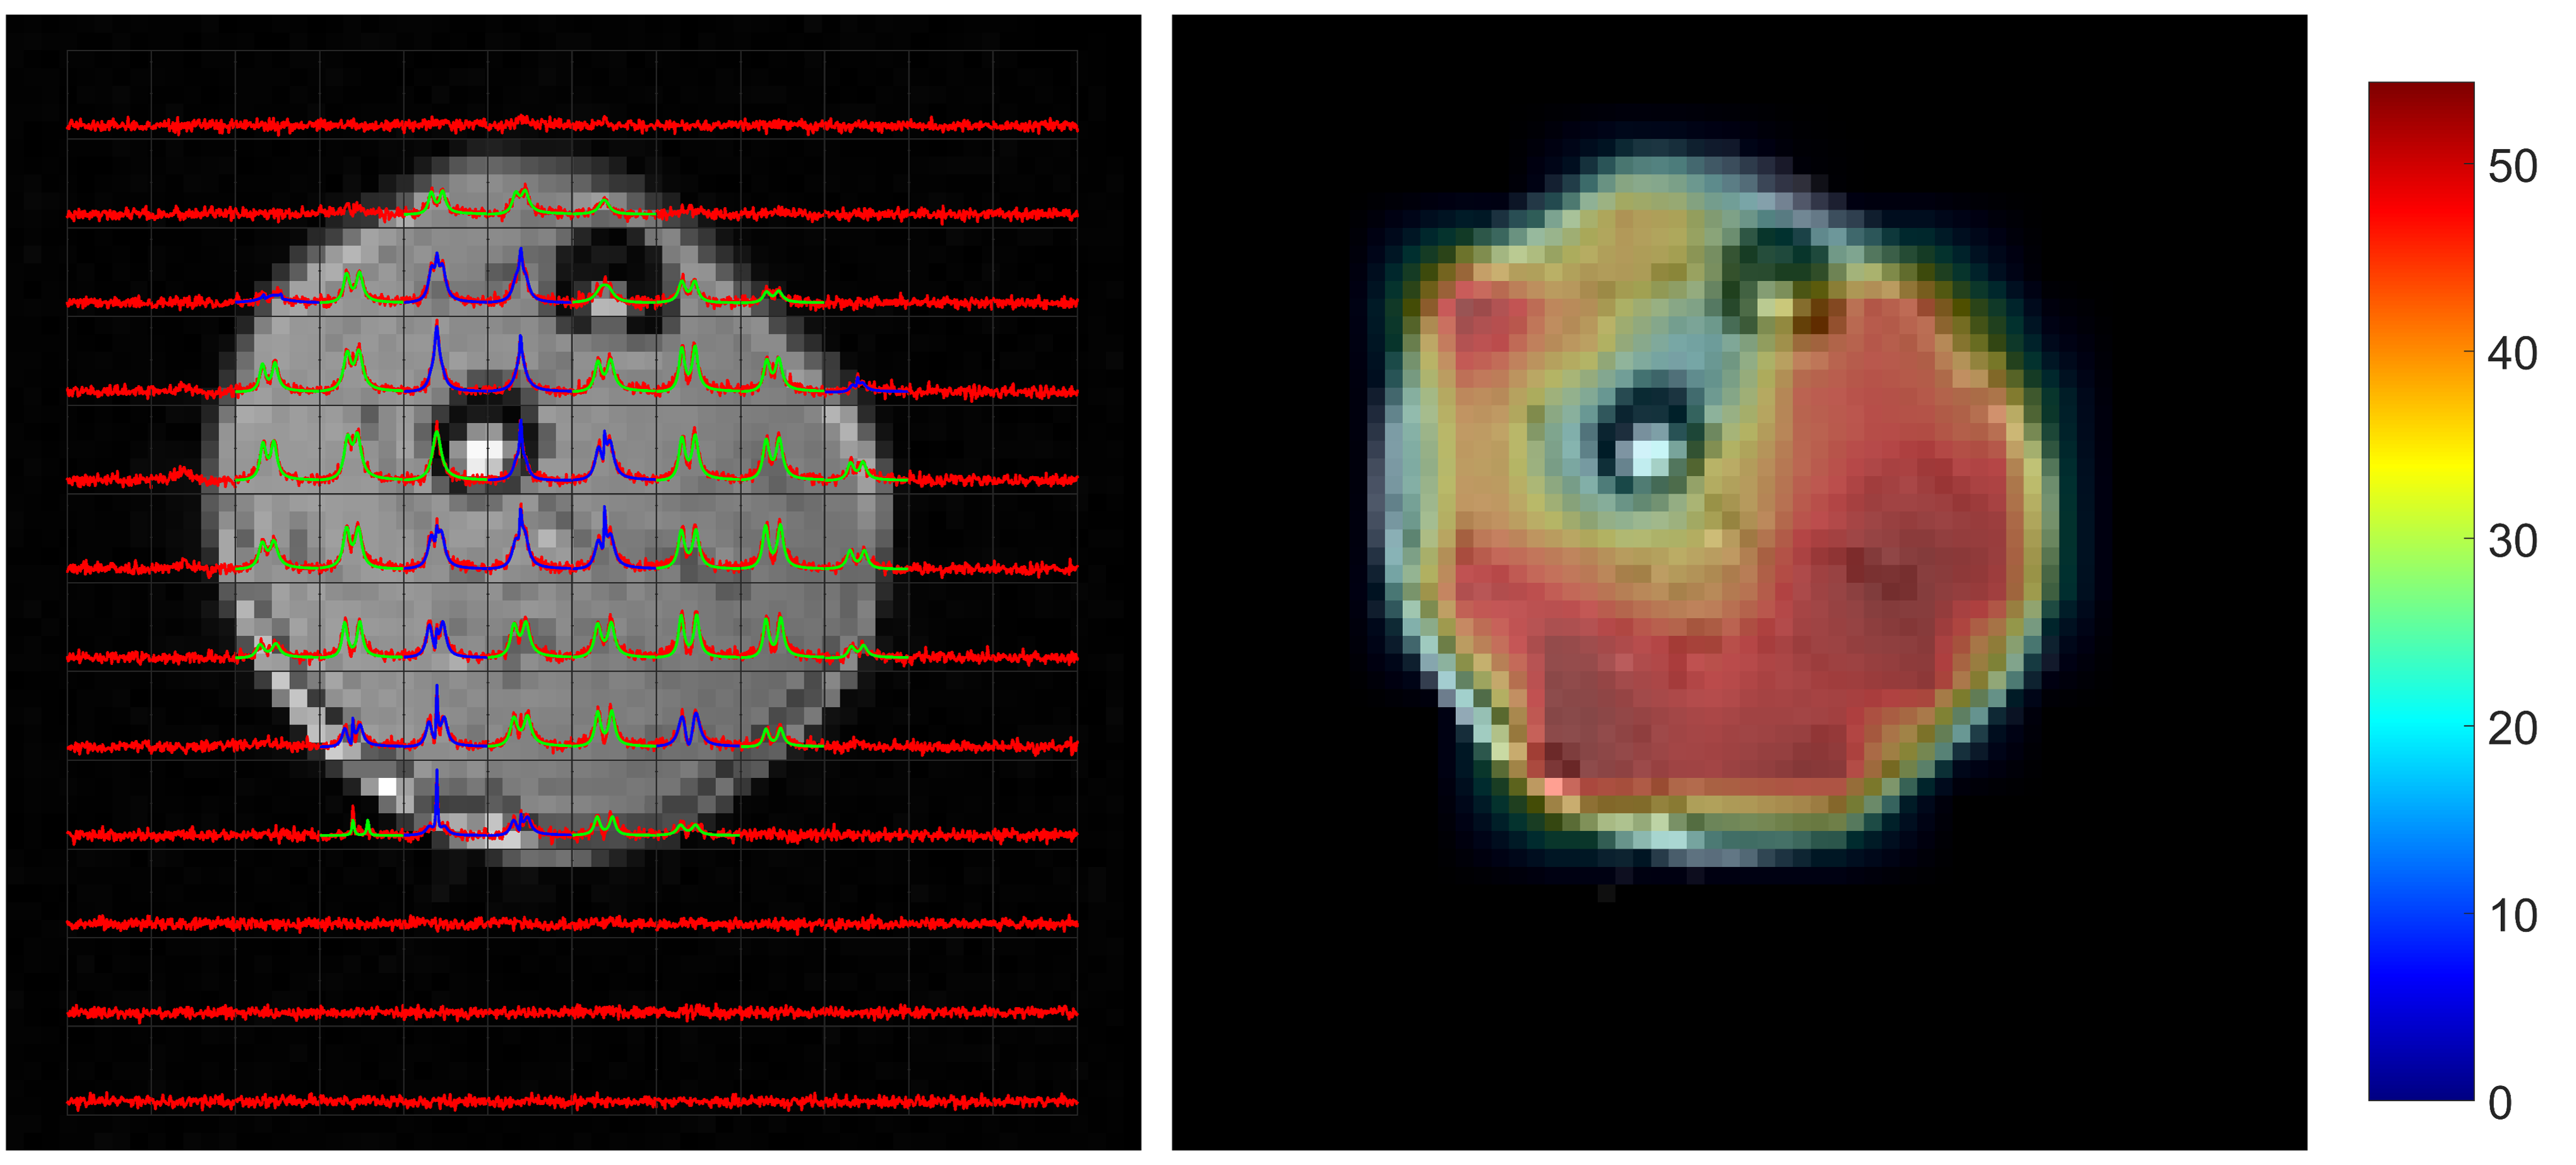
\includegraphics[width=1\textwidth]{Figures/D2O/Arm_A.png}
    \caption{Left: CSI spectra (red) overlayed onto a $^1$H GE image from participant A's left arm at an angle of 0 ${\circ}$ to the B0 field of a single slice, with fits of two Lorentzian peaks (green) and three Lorentzian peaks (blue). Right: Interpolated map of quadrupolar frequency splitting's overlayed onto the same $^1$H GE image from participant A's left arm. }
    \label{fig:D2O:Arm_A}
\end{figure}

\begin{figure}
    \centering
    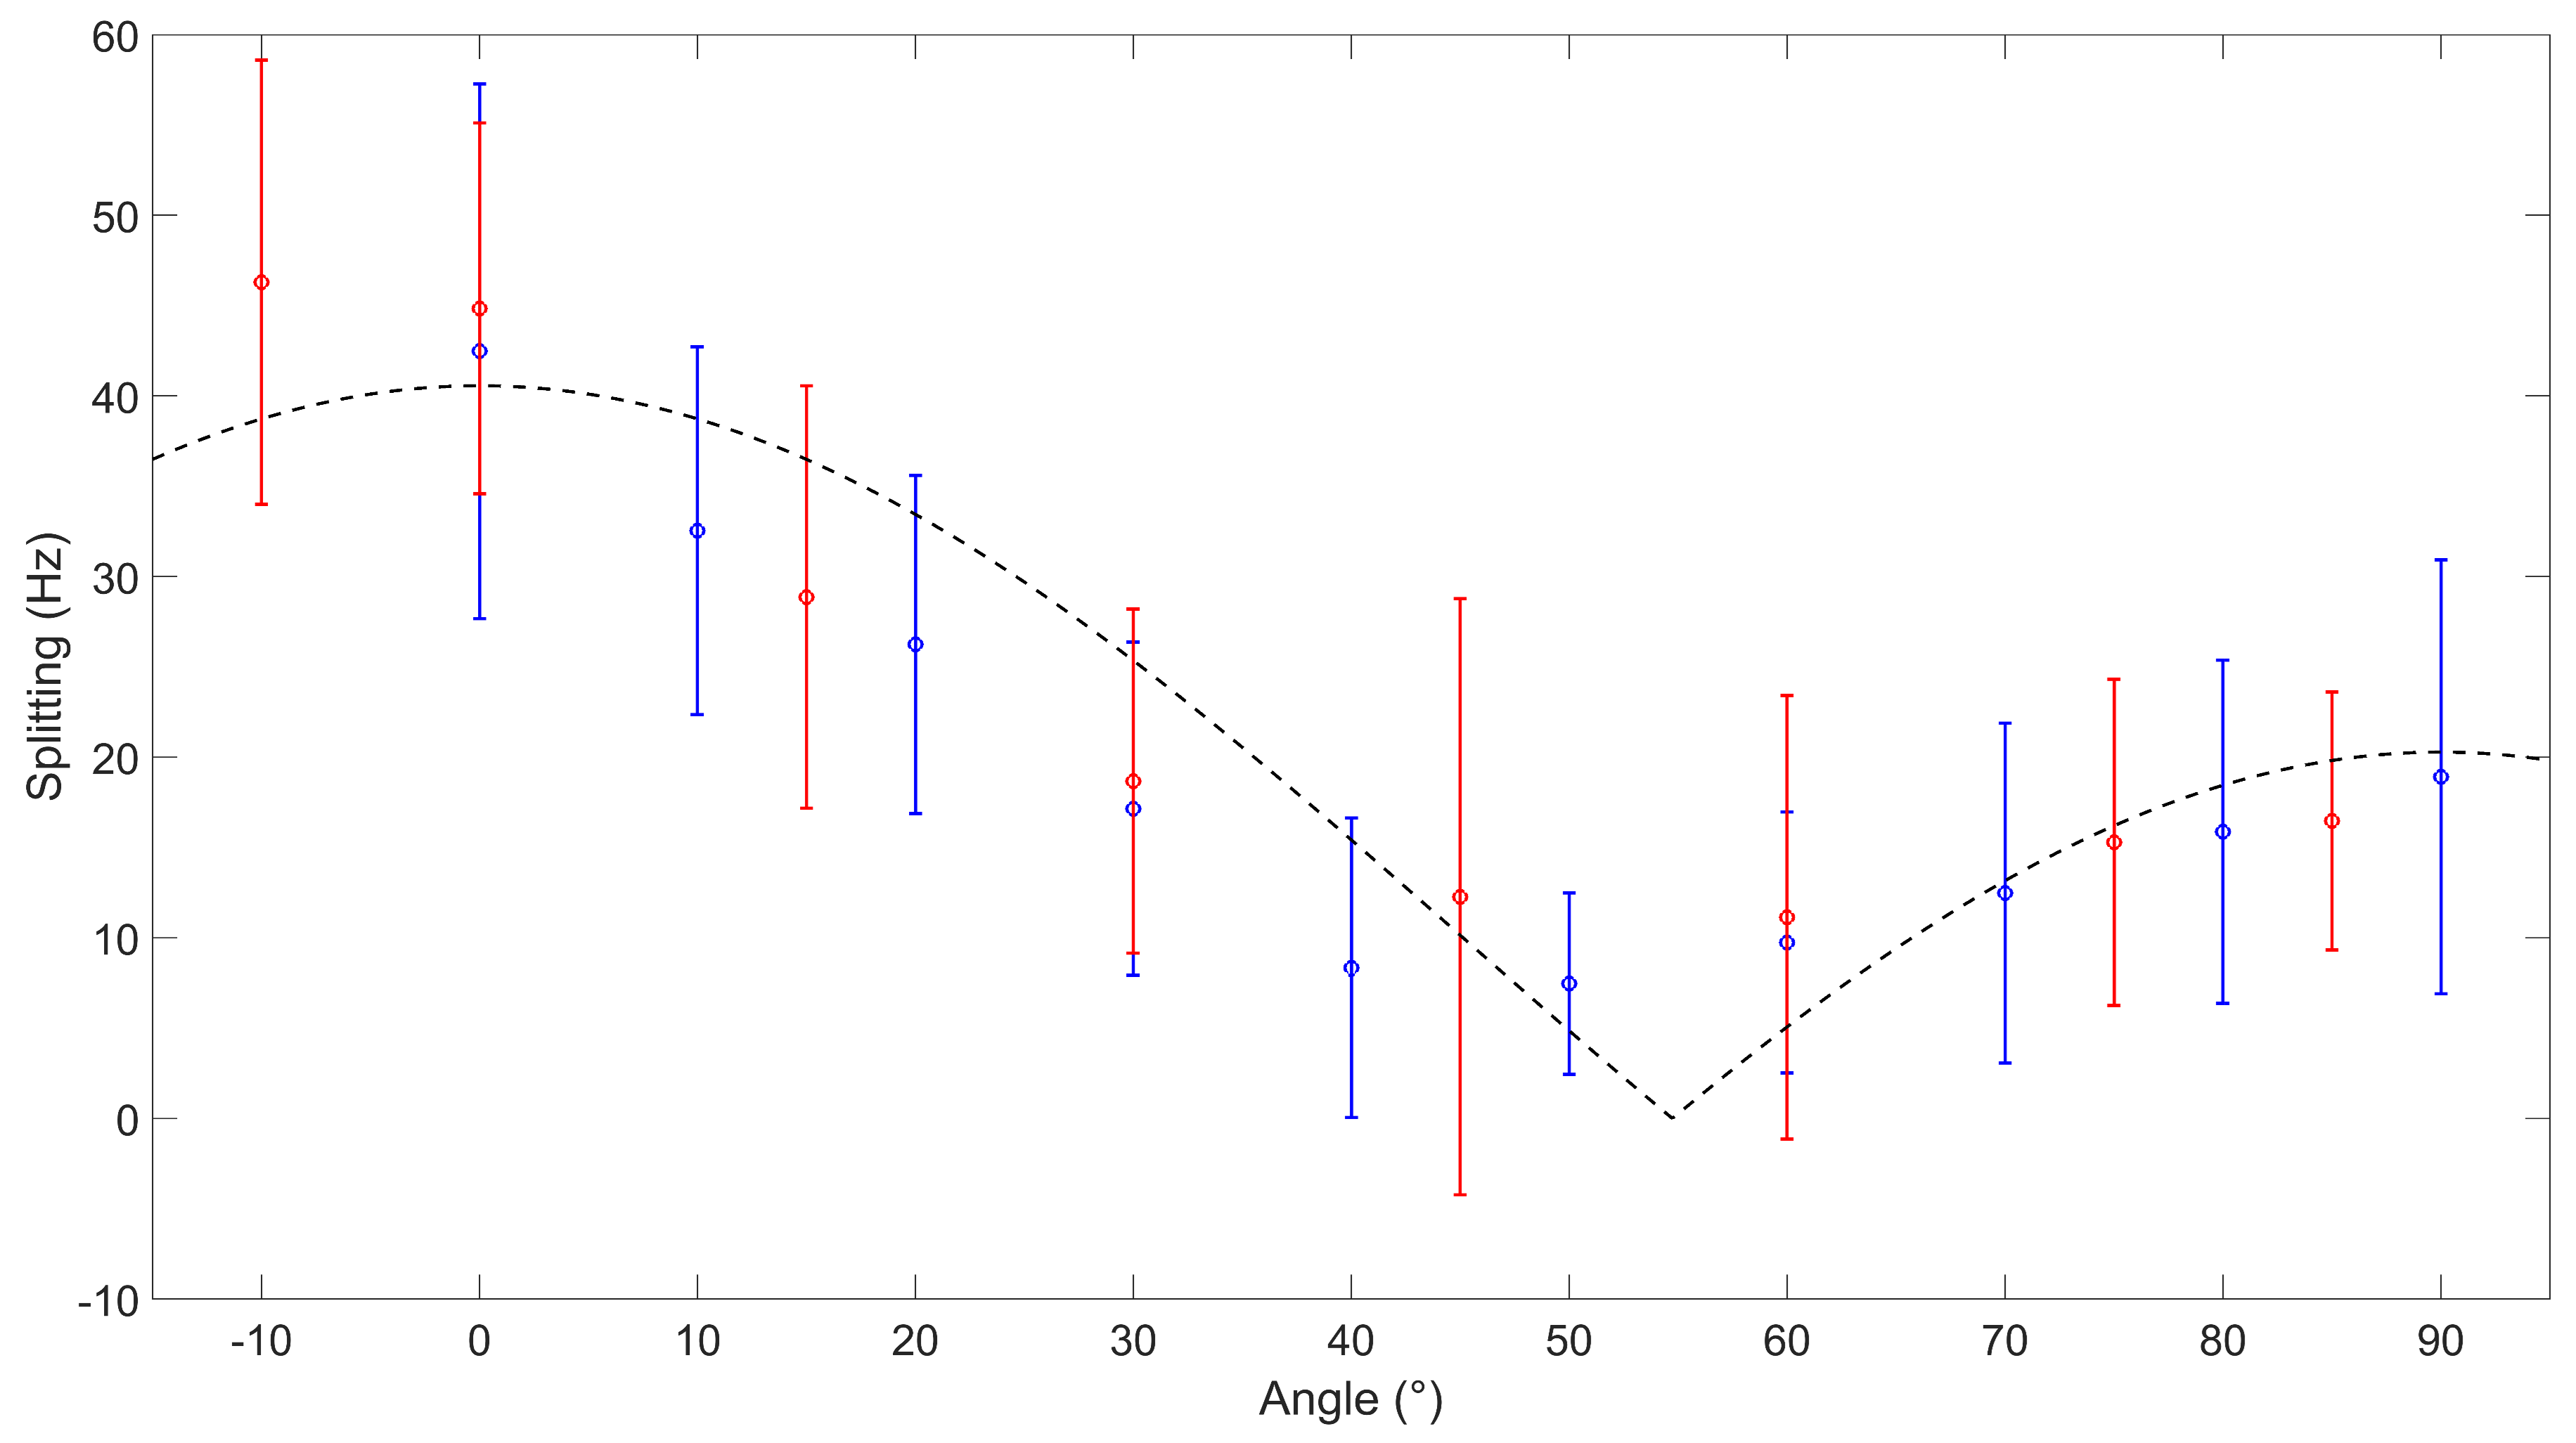
\includegraphics[width=1\textwidth]{Figures/D2O/Split_Angle.png}
    \caption{Graph Showing the variation of averaged quadrupolar frequency splittings of the arm against the angle to the B0 field they were positioned at, for partcipant A (blue) and B (red). Along with the fit (dotted black) of both participant's data to equation \ref{eqn.Angle}, the splitting magnitude of this fit is 38 $\pm$ 2 Hz.}
    \label{fig:D2O:Split_Angle}
\end{figure}

\section{Discussion}

\section{Conclusion}

% \printbibliography % Comment out main doc

\end{document}